\documentclass[12pt, letterpaper, twoside]{article}
\usepackage[utf8]{inputenc}
\usepackage[a4paper]{geometry}
\usepackage{array}
\usepackage{booktabs} % For prettier tables
\usepackage{multirow}
\usepackage{multicol}
\usepackage{ragged2e}
\usepackage{xcolor}
\usepackage{gensymb}
\usepackage{fullpage}
\usepackage{hyperref}
\usepackage{amsmath}
\usepackage{scrextend}
\usepackage{graphicx}
\usepackage{enumitem}

\graphicspath{ {./bilder/} }
\newcommand{\cfootnote}[1]{\footnote{\centering #1}}
\title{Ein $\underset{"}{\text{Numerus clausus}} $ für Venedig?}
\author{Simon Freiermuth \\ \href{mailto:simon@freiermuth.org}{simon@freiermuth.org}}
\date{\today}

\begin{document}

%\begin{titlepage}
\maketitle
%\end{titlepage}

\begin{flushleft}

\begin{enumerate}[label=\textbf{\arabic* .}]
    \item % 1.
    Definitionen:

    \begin{enumerate}[label=\textbf{\alph* )}]
	\item % a)
	Globalisierung:\\
	Globaler Austausch von Waren, Dienstleistungen und Touristen.

	\item % b)
	Gentrifizierung:\\
	Die Aufwertung/Verteuerung von heruntergekommenen Wohnquartieren mit guter Bausubstanz

	\item % c)
	Disneyisierung:\\
	Wenn gewisse Sehenswürdigkeiten oder ganze Städte von Touristen so überflutet werden, dass
	es seine ursprüngliche Charm verliert und alles auf die Touristen ausgerichtet ist, es ist alles
	nur für show. Wie im Disneyland.


    \end{enumerate}

    \item % 2.
    \begin{enumerate}[label=\textbf{\alph* )}]


	\item % a)
	Globalisierung:
	Nach Venedig kommen Touristen aus der ganzen Welt (30 Mio. p.a.), was im Vergleich zu rund 50000
	Einwohnern eine enorme Anzahl. Manche kommen sogar mit dem Velo. Pro Jahr kommen ca. 650
	Kreuzfahrtschiffe nach Venedig, dessen Passagiere rund 150 Mio. EUR pro Jahr in der Stadt ausgeben.
	Besucher aus der ganzen Welt drangen sich in den Gassen und Kanalen. Aufgrund seines
	Bekanntheitsgrades und der romantischen Verklärung hat jeder das Gefühl, einmal im Leben nach
	Venedig fahren zu müssen.

	\item % b)
	Gentrifizierung:
	In Venedig zu wohnen ist sehr teuer, unabhängig vom Quartier. Während der
	durchschnittliche Preis pro Quadratmeter für eine Wohnung in italienischen Städten im 2018
	rund 3550 EUR betrug, war es in Venedig über 5000 EUR. Auch wenn es
	wegen dem Handel der fleissig betrieben wird seit es Schiffe gibt, schon immer teuer war,
	hat der globale Tourismus die Preise explodieren lassen.
	Gemäss eines Luxusimmobilienmaklers sind rund 70\% der Käufer aus dem Ausland.
	Venedig zählte in den 60er jahren noch rund 170'000 Einwohner, hat jetzt aber nur noch 50'000.
	Viele Einheimische können sich die Immobilien nicht leisten, dies gilt auch für die Mieten.
	Kurzzeitige Vermietungen über Airbnb u.ä. sind wesentich lukrativer als langfristige vermietungen
	an Lokale.

	\item % c)
	Disneyisierung
	Die ganze Stadt ist eine Attraktion, wenn man sucht wird man kaum auf normale Sachen wie
	Lebensmittelläden stossen (eigene Erfahrung), die Stadt ist bis ins kleinste Detail auf die
	Touristen ausgerichtet, mit wenig Rücksicht auf die Einwohner. Wenn die Touristen Eintritt
	zahlen müssen wie es mit der Tagesgebühr der Fall ist, ist das Disneyland perfekt.
	(siehe \textbf{3.})


    \end{enumerate}

    \item % 3.
    Ein unfreiwilliger Lösungsansatz ist Covid19.
    Die Kanäle führen plötzlich sauberes Wasser, es gibt Quallen und Fische.

    Ein produktiver Lösungsansatz ist Kreuzfahrtschiffe zu verbieten.
    Jeden Tag fahren Kreuzfahrtschiffe mitten durch die Altstadt und bringen bis zu 5000 Passagiere pro
    Schiff mit. Wenn mehrere Schiffe auf einmal in Venedig sind dann kann es über 10'000 Kreuzfahrtpassagiere
    gleichzeitig in Venedig geben. das ist 10\% der Anzahl Einwohner.

    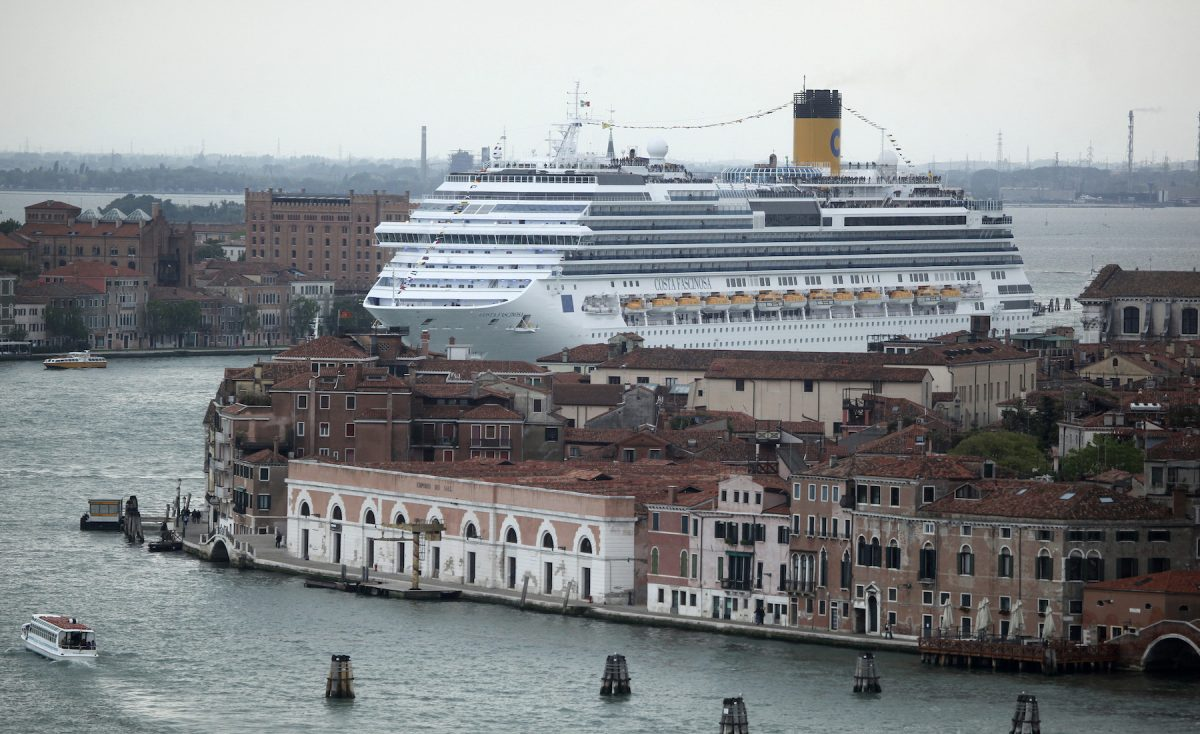
\includegraphics[scale=0.3]{boat}

    Eine Eintrittsgebühr wird auch diskutiert, das würde aber die Stadt endgültig zum Vergnügungspark machen.
    Diese Lösung würde es für Touristen die nicht so reich sind erschweren, und ungerechtigkeit schaffen.



\end{enumerate}

\end{flushleft}

\end{document}
